\chapter{Prerequisiti di Algebra}

Prima di iniziare a trattare gli argomenti principali del corso,
è necessario ripassare alcuni concetti di algebra alla base della teoria dei codici introducendone alcuni nuovi.

In particolare questo capitolo si concentra sulle strutture algebriche di semigruppi e monoidi e di loro proprietà utili per la teoria dei codici.

Inizialmente però, per addentrarci nelle definizioni delle suddette strutture algebriche, è necessario introdurre alcune notazioni preliminari, che verranno conservate per tutto il corso di questi appunti.

\section{Nozioni Preliminari}

Le lettere maiuscole \(A, B, X, Y \ldots\) indicheranno generalmente insiemi, che siano finiti o infiniti.
Per quanto riguarda gli insiemi numerici tradizionali, useremo:
\begin{itemize}
  \item \(\N = \set{0,1,2,\ldots}\) per i numeri naturali (incluso lo zero);
  \item \(\N_+ = \set{1,2,3,\ldots}\) per i numeri naturali positivi (escluso lo zero);
  \item \(\Z\) per i numeri interi;
  \item \(\Q\) per i numeri razionali;
  \item \(\R\) per i numeri reali.
\end{itemize}
Con eventuali notazioni aggiuntive a pedice per indicare sottoinsiemi particolari (ad esempio \(\R_{\geq 0}\) per i numeri reali non negativi).

Per ogni insieme \(X\), \(\mathcal{P}(X)\) denota l'insieme delle parti di \(X\), ovvero l'insieme di tutti i sottoinsiemi di \(X\) e \(\#X\) la sua cardinalità.
Gli elementi di tali insiemi saranno indicati con le lettere minuscole corrispondenti \(a,b,x,y \ldots\), in particolare con la lettera \(n\) a indicare un generico elemento naturale se non specificato diversamente.

\section{Semigruppi e Monoidi}
\begin{definition}{Semigruppo}
  Un \keyword{semigruppo} è una coppia \((S, \cdot)\) dove \(S\) è un insieme non vuoto e \(\cdot : S \times S \to S\) è un'operazione binaria associativa, ovvero:
  \[\forall a,b,c \in S, (a \cdot b) \cdot c = a \cdot (b \cdot c).\]
\end{definition}

Questa struttura algebrica è molto generica, imponendo solo l'associatività dell'operazione binaria.
Un esempio di semigruppo è dato da \((\N',+)\) dove l'operazione binaria è la somma tra numeri naturali positivi ordinaria.

\begin{definition}{Monoide}
  Un \keyword{monoide} \((M,\cdot,1_M)\) è un semigruppo \((M, \cdot)\) dotato di elemento neutro \(1_M\) per l'operazione binaria\footnote{Denotato semplicemente \(1\) in caso di non ambiguità del monoide di riferimento}, ovvero:
  \[\forall a \in M, a \cdot 1_M = 1_M \cdot a = a\]
\end{definition}

\begin{example}{}
  \begin{itemize}
    \item \((\N, +)\) è un monoide con elemento neutro \(0\).
    \item \((\N, \cdot)\) è un monoide con elemento neutro \(1\).
    \item Dato \(T\) insieme, sia \((\mathcal{P}(T), \cup, \emptyset)\) che \((\mathcal{P}(T), \cap, T)\) sono monoidi.
  \end{itemize}
  Gli esempi precedenti sono tutti monoidi commutativi (o abeliani), ovvero tali che:
  \[\forall a,b \in M, a \cdot b = b \cdot a.\]
  Un esempio di monoide non abeliano è, dato un insieme \(T\), il monoide delle funzioni totali da \(T\) in sé stesso \((T^{T}, \circ, id_T)\) dove l'operazione binaria è la composizione di funzioni e l'elemento neutro è la funzione identità su \(T\).
\end{example}

\subsection{Proprietà di monoidi e semigruppi}

Analizziamo ora alcune notazioni e proprietà di monoidi e semigruppi.

\begin{definition}[label=obs:power_notation]{}
  Dato \((M,\cdot,1_M)\) monoide, si ha che, \(\forall m \in M\), \(m^0 = 1_M\) e \(m^{n+1} = m \cdot m^n, \quad \forall n \geq 0\).
\end{definition}

\begin{definition}{Morfismi di semigruppi e monoidi}
  Siano \((S,\cdot)\) e \((T,*)\) semigruppi.
  Una funzione \(f: S \to T\) è un \keyword{morfismo di semigruppi} se:
  \[\forall a,b \in S, f(a \cdot b) = f(a) * f(b).\]
  Se \(S\) e \(T\) sono monoidi, \(f\) è un \keyword{morfismo di monoidi} se è un morfismo di semigruppi e:
  \[f(1_S) = 1_T.\]
  Se \(f\) è iniettiva, si dice che è un \keyword{monomorfismo}, se è suriettiva si dice che è un \keyword{epimorfismo}, se è biunivoca si dice che è un \keyword{isomorfismo}.
  In quest'ultimo caso, i due semigruppi (o monoidi) si dicono isomorfi.
\end{definition}

\begin{example}{}
  Consideriamo i monoidi \((\N, +, 0)\) e \((\N, \cdot, 1)\).
  La funzione 
  \[f: \N \to \N\]
  \[f:n \mapsto f(n) = 2^n\]
  è un monomorfismo tra i due monoidi.
  Infatti,
  \[f(n+m) = 2^{n+m} = 2^n \cdot 2^m = f(n) \cdot f(m)\]
  \[ f(0) = 2^0 = 1\]
  Tuttavia, \(f\) non è un epimorfismo, poiché non è suriettiva (ad esempio, non esiste \(n \in \N\) tale che \(f(n) = 3\)).
\end{example}

\begin{definition}{Sottosemigruppo e Sottomonoide}
  Sia \((S,\cdot_S)\) un semigruppo.
  \(T \subseteq S\) è un \keyword{sottosemigruppo} di \(S\) (\(T \leq S\)), se \(T\) è chiusa rispetto all'operazione binaria di \(S\), ovvero:
  \[\forall a,b \in T, a \cdot_S b \in T\]
  Dato \((M,\cdot_M,1_M)\) è un monoide, \(N \subseteq M\) è un \keyword{sottomonoide} di \(M\) (\(N \leq M\)) se:
  \begin{itemize}
    \item \(N\) è un sottosemigruppo di \(M\);
    \item \(1_M \in N\).
  \end{itemize}
\end{definition}

Dato un qualsiasi semigruppo \((S,\cdot)\), è possibile costruire un semigruppo sul suo insieme delle parti \(\mathcal{P}(S)\) indotto dall'operazione binaria di \(S\).
\begin{definition}{Semigruppo delle parti}
  Sia \((S,\cdot)\) un semigruppo.
  Definiamo l'operazione binaria \(\circ\) su \(\mathcal{P}(S)\) come:
  \[\forall X,Y \in \mathcal{P}(S), X \circ Y = \set{x \cdot y}[ x \in X, y \in Y].\]
\end{definition}
Tale costruzione è estendibile anche a un qualsiasi monoide \((M,\cdot,1_M)\), usando come elemento neutro l'insieme \(\set{1_M}\).

Questo semigruppo (o monoide) delle parti è particolarmente rilevante, poiché, grazie alle notazioni introdotte nella \Cref{obs:power_notation}, è possibile definire le potenze di un qualsiasi sottoinsieme \(Y \subseteq S\).

Tale notazione permette di formulare in modo più compatto la chiusura di un sottoinsieme \(Y\) di un semigruppo.
  \[(\forall a,b \in T, a \cdot_S b \in T)\iff (Y^2 \subseteq Y).\]

\begin{definition}{Sottostruttura generata}
  Sia \((S,\cdot)\) un semigruppo e \(Y \subseteq S\).
  Definiamo il \keyword{sottosemigruppo} di \(S\) generato da \(Y\) come:
  \[Y^+ = Y \cup Y^2 \cup Y^3 \cup \cdots = \bigcup_{n=1}^{\infty} Y^n\]
  l'insieme di tutte le possibili combinazioni finite di elementi di \(Y\) tramite l'operazione binaria di \(S\).

  Dato \((M,\cdot_M,1_M)\) monoide, è possibile aggiungere la potenza zero, definendo il \keyword{sottomonoide} di \(M\) generato da \(Y\) come:
  \[Y^* = \set{1_S} \cup Y^+ = \bigcup_{n=0}^{\infty} Y^n.\]
\end{definition}

\begin{definition}{Base di un semigruppo (monoide)}
  Sia \(S\) un semigruppo (monoide).
  Una \keyword{base} di \(S\) è un sottoinsieme \(X \subseteq S\) che gode di \emph{univoca fattorizzazione}, ovvero che dati \(\forall x_1,x_2,\ldots,x_n,x_1',x_2',\ldots,x_m' \in X\) si ha che:
  \[x_1 x_2 \ldots x_n = x_1' x_2' \ldots x_m' \implies n=m \land x_1 = x_1' \land x_2 = x_2' \land \ldots \land x_n = x_n'\]
\end{definition}
In altre parole, ogni elemento di \(X^{+}\) si fattorizza in un unico modo come prodotto di elementi di \(X\).

\begin{observation}[label=obs:no_neutral_in_base]{}
  Per definizione di base, nessuna base di un monoide può contenere l'elemento neutro.
  Infatti, se \(1_M \in X\), \(\forall x \in X\) si ha che \(1_M \cdot x = x\), quindi ogni elemento di \(X^{+}\) si fattorizza in un modo non univoco.
\end{observation}

\begin{definition}{Semigruppi e monoidi liberi}
  Data \(X \subseteq S\) base di un semigruppo \(S\), si dice che \(S\) è \keyword{libero} se \(S = X^{+}\).
  Analogamente, dato \(X \subseteq M\) base di un monoide \(M\), si dice che \(M\) è \keyword{libero} se \(M = X^{*}\).
\end{definition}
Un modo meno formale ma più intuitivo di definire un semigruppo (monoide) libero è quella di considerarlo il semigruppo (monoide) con la minor quantità di vincoli possibile, ovvero solo quelli imposti dalla definizione di semigruppo (monoide).
La struttura è \emph{libera} poiché non ha vincoli aggiuntivi che la limitano, essendo dunque la più generale possibile dato l'insieme sottostante.
Tale proprietà di generalità verrà formalizzata più avanti tramite una proprietà universale.
\begin{proposition}{Unicità della base in un semigruppo (monoide) libero}
  Sia \(S\) un semigruppo libero, allora l'unica base di \(S\) è \(S \setminus S^2\), ovvero l'insieme degli elementi di \(S\) che non sono esprimibili come prodotto di altri elementi di \(S\).
  Analogamente, sia \(M\) un monoide libero, allora l'unica base di \(M\) è \((M\setminus \{1_M\}) \setminus {(M\setminus \{1_M\})}^2\).
\end{proposition}

\begin{theorem}{Proprietà universale dei monoidi (semigruppi) liberi}
  Sia \(M\) un monoide con \(X \subseteq M\). Allora \(M\) è libero di base \(X\) se e solo se, per ogni monoide \(M'\) e ogni applicazione \(f: X \to M'\), esiste un unico morfismo di monoidi \(\bar{f}: M \to M'\) tale che \(\hat{f}_{|_X} = f\), ovvero tale che il seguente diagramma commuta:
  \begin{center}
      \begin{tikzcd}[column sep=huge, row sep=huge, cells={nodes={scale=1.2, transform shape}}]
        X \arrow[r, "f"] \arrow[d, hook,"i"] & M' \\ %chktex 18 
        M \arrow[ru, dashed, "\exists!\bar{f}"'] & %chktex 18
      \end{tikzcd}
  \end{center}
  Vale a dire che \(\bar{f} \circ i = f\), dove \(i: X \hookrightarrow M\) è l'inclusione di \(X\) in \(M\).\footnote{È possibile vedere \(i\) anche come la riduzione dell'identità di \(M\) a \(X\), ovvero \(i = id_{M|_X}\).}
  Tale formulazione ha carattere algebrico-universale e quindi può essere estesa anche ai semigruppi, oltre che a qualsiasi famiglia di algebre dello stesso tipo, quali per esempio i gruppi.
\end{theorem}

In altre parole, esiste un unico morfismo \(\bar{f}\) da \(M\) a \(M'\) che estende \(f\) morfismo da \(X\) a \(M'\); se così non è, allora \(M\) non è libero di base \(X\).
È importante notare che la proprietà universale, dato un monoide \(M\) e una sua base \(X\) vale \emph{per ogni monoide \(M'\)}, e quindi in particolare anche per \(M' = M\).
Da questa particolare circostanza è facile ricavare che \(id_M: M \to M\) è l'unico morfismo da \(M\) a \(M\) che estende \(id_X\).

\begin{corollary}{}
  Sia \(M\) monoide libero di base \(X\) e \(M'\) monoide libero di base \(X'\).
  Se \(\#X = \#X'\), allora \(M\) e \(M'\) sono isomorfi.
\end{corollary}

\begin{proof}
  Per dimostrare tale corollario sarà sufficiente mostrare che è possibile costruire un morfismo biettivo (isomorfismo) tra \(M\) e \(M'\)
  Essendo le basi equipotenti, esiste una biiezione \(g: X \leftrightarrow X'\).
  Consideriamo l'applicazione \(f = i' \circ g : X \to M'\), dove \(i': X' \hookrightarrow M'\), ovvero l'inclusione di \(X'\) in \(M'\).
  Per la proprietà universale, esiste un unico morfismo di monoidi \(\bar{f}: M \to M'\) tale che \(\bar{f}_{|_X} = f\).
  Analogamente, sia \(f'= i \circ g^{-1} : X' \to M\) e sia \(\bar{f'}: M' \to M\) l'unico morfismo di monoidi tale che \(\bar{f'}_{|_{X'}} = f'\).
  Si ha che \(\bar{f'} \circ \bar{f}: M \to M\) è un morfismo di monoidi che estende \(id_X\), ovvero:
  \[\forall x \in X, \bar{f'} (\bar{f}(x)) = \bar{f'}(g(x))= g^{-1}(g(x))= x\]
  Come detto precedentemente però \(id_M\) è l'unico morfismo di monoidi da \(M\) in sé stesso che estende \(id_X\), dunque necessariamente si ha che \(\bar{f'} \circ \bar{f} = id_M\)
  Dalla definizione di biettività abbiamo che \(\bar{f} = \bar{f'}^{-1} \), ovvero che \(\bar{f}\) è un isomorfismo tra \(M\) e \(M'\). 
\end{proof}
Questo corollario mostra che, a meno di isomorfismi, il monoide libero \(A^*\) è l'unico monoide libero con base di cardinalità \(\#A\).

Dato un monoide libero \(M\) è possibile definire un morfismo di lunghezza delle parole.
\begin{definition}{Morfismo di lunghezza}
  Sia \(M\) un monoide libero di base \(X\).
  Il \keyword{morfismo di lunghezza} è \(|\;|: M \to(\N,+,0)\) tale che \[\forall x \in X, |x| = 1\]
\end{definition}

\begin{observation}{}
  È importate notare che il morfismo di lunghezza è ben definito per ogni valore di \(M\), poiché ogni elemento di \(M\) si fattorizza in modo univoco come prodotto di elementi di \(X\).
  Non fosse stato così, non sarebbe possibile definire in modo univoco la lunghezza di un elemento di \(M\) a partire dagli elementi della sua base.
\end{observation}

\begin{lemma}[label=lem:levi]{Levi}
  Sia \(M\) un monoide libero, \(m_1,m_2,m_3,m_4 \in M\) tali che \(m_1m_2=m_3m_4 \text{ e } |m_1| \geq |m_3|\).
  Allora \(\exists v \in M: m_1 = m_3v \land vm_2 = m_4\)
\end{lemma}

\begin{proof}
  Chiamiamo \(w\) la parola comune \(m_1m_2 = m_3m_4\).
  Possiamo rappresentare la sua fattorizzazione in \(m_1m_2\) come:
  \begin{figure}[H]
    \centering
    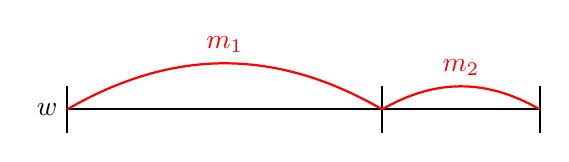
\begin{tikzpicture}
      \coordinate (A) at (0,0);
      \coordinate (B) at (6,0);
      \draw[thick] (A) -- (B);
      \foreach \x in {0,4,6}{
        \coordinate (P\x) at (\x,0);
        \draw[thick] (P\x) -- ++(0,-0.3);
        \draw[thick] (P\x) -- ++(0,0.3);
      }
      \node[left] at (A) {\(w\)};
      \draw[thick, red, bend left] (A) to node[midway, above, red] {\(m_1\)} (P4);
      \draw[thick, red,bend left] (P4) to node[midway, above, red] {\(m_2\)} (P6);
    \end{tikzpicture}
  \end{figure}
  e la fattorizzazione in \(m_3m_4\) come:
  \begin{figure}[H]
    \centering
    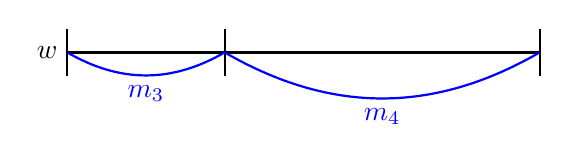
\begin{tikzpicture}
      \coordinate (A) at (0,0);
      \coordinate (B) at (6,0);
      \draw[thick] (A) -- (B);
      \foreach \x in {0,2,6}{
        \coordinate (P\x) at (\x,0);
        \draw[thick] (P\x) -- ++(0,-0.3);
        \draw[thick] (P\x) -- ++(0,0.3);
      }
      \node[left] at (A) {\(w\)};
      \draw[thick, blue,bend right] (A) to node[midway, below, blue] {\(m_3\)} (P2);
      \draw[thick, blue,bend right] (P2) to node[midway, below, blue] {\(m_4\)} (P6);
    \end{tikzpicture}
  \end{figure}
  Se \(\abs{m_1} = \abs{m_3}\), dall'ipotesi che \(M\) è libero segue che \(m_1 = m_3\) e \(m_2 = m_4\).
  Questo perché, non fossero uguali, si avrebbe una doppia fattorizzazione di \(w\), in contraddizione con la definizione di base.
  Il teorema in questo caso è verificato ponendo \(v = \varepsilon\).

  Nel caso \(\abs{m_1} > \abs{m_3}\) invece, il punto di divisione tra \(m_1\) e \(m_2\) si trova a destra del punto di divisione tra \(m_3\) e \(m_4\).
  Di conseguenza, è possibile sovrapporre le rappresentazioni precedenti come segue:
  \begin{figure}[H]
    \centering
    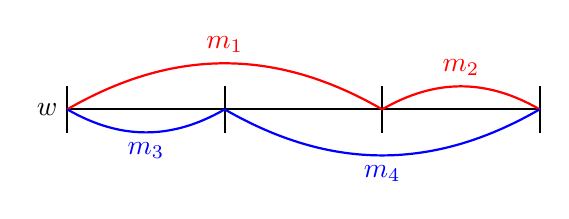
\begin{tikzpicture}
      \coordinate (A) at (0,0);
      \coordinate (B) at (6,0);
      \draw[thick] (A) -- (B);
      \foreach \x in {0,2,4,6}{
        \coordinate (P\x) at (\x,0);
        \draw[thick] (P\x) -- ++(0,-0.3);
        \draw[thick] (P\x) -- ++(0,0.3);
      }
      \node[left] at (A) {\(w\)};
      \draw[thick, red, bend left] (A) to node[midway, above, red] {\(m_1\)} (P4);
      \draw[thick, red,bend left] (P4) to node[midway, above, red] {\(m_2\)} (P6);
      \draw[thick, blue,bend right] (A) to node[midway, below, blue] {\(m_3\)} (P2);
      \draw[thick, blue,bend right] (P2) to node[midway, below, blue] {\(m_4\)} (P6);
    \end{tikzpicture}
  \end{figure}
  Chiamando \(v\) la parola compresa tra i due punti di divisione si ha che \(m_1 = m_3v\) e \(vm_2 = m_4\).
  Anche in questo caso, se una delle due uguaglianze non fosse verificata, si avrebbe una doppia fattorizzazione di \(w\), in contraddizione con la definizione di base.
  \begin{figure}
    \centering
    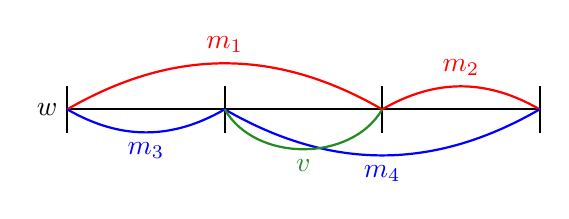
\begin{tikzpicture}
      \coordinate (A) at (0,0);
      \coordinate (B) at (6,0);
      \draw[thick] (A) -- (B);
      \foreach \x in {0,2,4,6}{
        \coordinate (P\x) at (\x,0);
        \draw[thick] (P\x) -- ++(0,-0.3);
        \draw[thick] (P\x) -- ++(0,0.3);
      }
      \node[left] at (A) {\(w\)};
      \draw[thick, red, bend left] (A) to node[midway, above, red] {\(m_1\)} (P4);
      \draw[thick, red,bend left] (P4) to node[midway, above, red] {\(m_2\)} (P6);
      \draw[thick, blue,bend right] (A) to node[midway, below, blue] {\(m_3\)} (P2);
      \draw[thick, blue,bend right] (P2) to node[midway, below, blue] {\(m_4\)} (P6);
      \draw[thick, ForestGreen, bend right=60] (P2) to node[midway, below, ForestGreen] {\(v\)} (P4);
    \end{tikzpicture}
  \end{figure}
\end{proof}

\begin{definition}[label=def:quotient_sets]{Insiemi quoziente}
  Siano \(Y,Z \subseteq M\) monoide. Definiamo gli insiemi quoziente destro e sinistro come:
  \begin{equation}
    \begin{aligned}
      Y^{-1}Z &= \set{m \in M}[ \exists y \in Y, ym \in Z]\\
      ZY^{-1} &= \set{m \in M}[ \exists y \in Y, my \in Z]
    \end{aligned}
  \end{equation}
\end{definition}

In altre parole, possiamo vedere $Y^{-1}Z$ come l'insieme di quegli $m\in M$ che, messi a destra di un $y\in Y$, stanno in $Z$.

\begin{theorem}[label=thm:schützenberger_monoids]{Schützenberger sui sottomonoidi liberi}
  Sia \(M\) libero e \(N \leq M\). Allora \(N \text{ è libero } \iff N^{-1}N \cap NN^{-1} \subseteq N\)
\end{theorem}
In altre parole questo teorema ci dice che \(N\) sottomonoide di \(M\) libero è a sua volta libero se e solo se ogni parola di \(M\) che completa sia a destra che a sinistra parole di \(N\) sia a sua volta inclusa in \(N\).
Tale formulazione può essere espressa formalmente come:
\[N \text{ libero } \iff \left(\forall m \in M (\exists n_1,n_2,n_3,n_4( n_1m=n_2 \land mn_3=n_4) \implies m \in N)\right)\]

\begin{observation}{}
  Se \(N\leq M\) necessariamente \(N \subseteq N^{-1}N \cap NN^{-1}\) poiché tutte le parole di \(N\) completano sia a destra che a sinistra la parola vuota per formare se stesse.
  Di conseguenza il teorema può essere riformulato equivalentemente come:
  \begin{theorem}{Schützenberger alt.}
    Sia \(M\) libero e \(N \leq M\). Allora \(N \text{ è libero } \iff N^{-1}N \cap NN^{-1} = N\)
  \end{theorem}
  In altre parole un sottomonoide di un monoide libero è esso stesso libero se non contiene più del necessario.
\end{observation}

\begin{proof}[\extrasymbol{} Dimostrazione di~\ref{thm:schützenberger_monoids}]
  In caso uno qualsiasi tra \(n_1,n_2,n_3,n_4 \in N\) e \(m \in M\) sia l'elemento neutro \(1_M\) la doppia implicazione è verificata in maniera banale.
  Assumendo dunque che tutti gli elementi coinvolti siano diversi da \(1_M\) andiamo a dimostrare i due versi della doppia implicazione:
  \begin{description}
    \item[\q{\(\implies\)}]
      Supponiamo che \(N\) sia libero, e siano \(m \in M, n_1,n_2,n_3,n_4 \in N\) tali che\footnote{Possiamo assumere che esistano, poiché altrimenti il predicato che vogliamo verificare sarebbe banalmente vero per implicazione vacua} \(n_1m = n_2\) e \(mn_3 = n_4\).
      Si ha dunque che
      \[n_1 m n_3 = n_2 n_3 \implies n_1 n_4 = n_2 n_3\]
      Sia dunque \(X\) base di \(N\). Siano \(a_1, \ldots, a_h, b_1, \ldots, b_k, c_1, \ldots, c_i, d_1, \ldots, d_j \in X\) tali che
      \[n_1 = a_1 \ldots a_h, n_2 = b_1 \ldots b_k, n_3 = c_1 \ldots c_i, n_4 = d_1 \ldots d_j\]
      Dall'uguaglianza precedente segue che
      \[a_1 \ldots a_h d_1 \ldots d_j = b_1 \ldots b_k c_1 \ldots c_i\]
      Essendo \(N\) libero, tale fattorizzazione è unica, dunque necessariamente \(h+j = k+i\) e che \(a_1 = b_1\).
      
      Possiamo dunque rappresentare tale parola come segue:
      \begin{figure}[H]
        \centering
        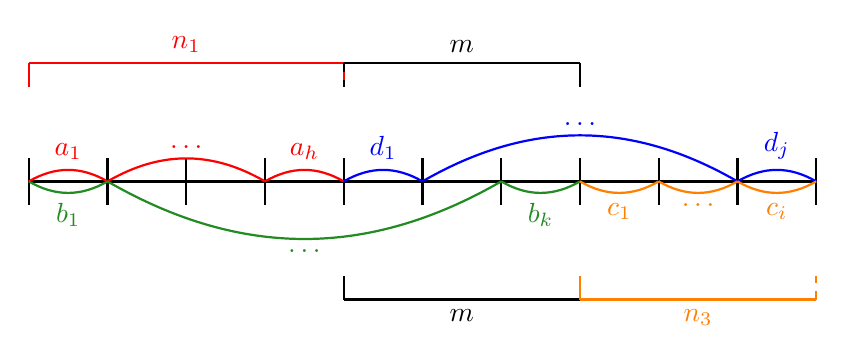
\begin{tikzpicture}
          \foreach \x in {0,1,2,3,4,5,6,7,8,9,10}{
            \coordinate (P\x) at (\x,0);
            \draw[thick] (P\x) -- ++(0,-0.3);
            \draw[thick] (P\x) -- ++(0,0.3);
            }
          \draw[thick] (P0) -- (P10);
            % \node[left] at (A) {\(n_1 m n_3 = n_2 n_3\)};
          \draw[thick, red, bend left] (P0) to node[midway, above, red] {\(a_1\)} (P1);
          \draw[thick, red, bend left] (P1) to node[midway, above, red] {\(\ldots\)} (P3);
          \draw[thick, red,bend left] (P3) to node[midway, above, red] {\(a_h\)} (P4);
          \draw[thick, blue,bend left] (P4) to node[midway, above, blue] {\(d_1\)} (P5);
          \draw[thick, blue,bend left] (P5) to node[midway, above, blue] {\(\ldots\)} (P9);
          \draw[thick, blue,bend left] (P9) to node[midway, above, blue] {\(d_j\)} (P10);

          \draw[thick, ForestGreen, bend right] (P0) to node[midway, below, ForestGreen] {\(b_1\)} (P1);
          \draw[thick, ForestGreen, bend right] (P1) to node[midway, below, ForestGreen] {\(\ldots\)} (P6);
          \draw[thick, ForestGreen,bend right] (P6) to node[midway, below, ForestGreen] {\(b_k\)} (P7);
          \draw[thick, orange,bend right] (P7) to node[midway, below, orange] {\(c_1\)} (P8);
          \draw[thick, orange,bend right] (P8) to node[midway, below, orange] {\(\ldots\)} (P9);
          \draw[thick, orange,bend right] (P9) to node[midway, below, orange] {\(c_i\)} (P10);

          \draw[thick, red] (0,1.5) to node[midway, above, red] {\(n_1\)} (4,1.5);
          \draw[thick,red] (0,1.5) -- ++(0,-0.3);
          \draw[thick, red] (4,1.5) -- ++(0,-0.3);
          \draw[thick] (4,1.5) to node[midway, above] {\(m\)} (7,1.5);
          \draw[thick,dashed] (4,1.5) -- ++(0,-0.3);
          \draw[thick] (7,1.5) -- ++(0,-0.3);

          \draw[thick] (4,-1.5) to node[midway, below] {\(m\)} (7,-1.5);
          \draw[thick] (4,-1.5) -- ++(0,+0.3);
          \draw[thick] (7,-1.5) -- ++(0,+0.3);
          \draw[thick, orange] (7,-1.5) to node[midway, below, orange] {\(n_3\)} (10,-1.5);
          \draw[thick, orange,dashed] (10,-1.5) -- ++(0,+0.3);
          \draw[thick, orange] (7,-1.5) -- ++(0,+0.3);
          
        \end{tikzpicture}
      \end{figure}
    
      Si ha dunque che \(m = b_{h+1}\ldots b_k = d_1 \ldots d_{j-i}\), e dunque \(m \in N\).
    \item[\q{\(\impliedby\)}]
      Supponiamo che \(N^{-1}N \cap NN^{-1} \subseteq N\).
      Sia inoltre \(X = (N\setminus \set{1})\setminus{(N\setminus \set{1})}^2\) e supponiamo per assurdo che \(X\) non sia una base di \(N\).
      Esistono dunque \(x_1, \ldots, x_i, x_1', \ldots, x_j' \in X\) tali che \(x_1\ldots x_i = x_1'\ldots x_j'\) con \(x_1 \neq x_1'\).
      Senza perdita di generalità, supponiamo che \(\abs{x_1} < \abs{x_1'}\).
      Per il lemma di Levi (\ref{lem:levi}) esiste \(v \in M\) tale che \(x_1' = x_1 v\) e \(x_2 \ldots x_i = v x_2' \ldots x_j'\).
      Ponendo \(m = v, n_1 = x_1, n_2 = x_1', n_3 = x_2'\ldots x_j', n_4 =  x_2 \ldots x_i\), dall'ipotesi segue che \(v \in N\).
      Ma \(x_1 \in X \implies x_1 \in N\), e dunque \(x_1' = x_1 v \in {(N\setminus\set{1})}^2\), in contraddizione con la definizione di \(X\).
      Dunuque \(X\) è una base di \(N\), e \(N\) è libero.
  \end{description}
\end{proof}

% Esempio di sottomonoide non libero è ad esempio qualsiasi monoide generato da un qualsiasi \(X \subseteq \N\setminus {1}\) ristpetto all'addizione.

\begin{definition}{Sottomoide unitario}
  Dato \(M\) monoide, \(N \leq M\) è detto \keyword{unitario a sinistra} (rispettivamente a destra) se:
  \[N^{-1}N \subseteq N \text{ sx}\]
  \[NN^{-1} \subseteq N \text{ dx}\]
  \(N\) si dice \keyword{unitario} se è unitario a sinistra o a destra.
\end{definition}

% se è unitario è libero non viceversa
Da tale definizione e dal teorema~\ref{thm:schützenberger_monoids} segue che, dato \(M\) monoide libero, se  \(N \leq M\) è unitario, allora è libero.


Finita la parte introduttiva su gli strumenti matematici necessari,
possiamo finalmente addentrarci nel primo capitolo: i codici.